\section{Diverses}
\subsection{Partialbruchzerlegung}
	\[f(x)=\frac{x^2+20x+149}{x^3+4x^2-11x-30} \Rightarrow \; \begin{array}{l}\text{Nenner faktorisieren mit}\\
	\text{Hornerschema, Binom, etc.}\end{array} \Rightarrow
	x^{3}+4x^{2}-11x-30=(x+2)(x^{2}+2x-15)=(x+2)(x+5)(x-3)\] Ansatz:
	\[f(x)=\frac{x^2+20x+149}{x^3+4x^2-11x-30}=\frac{A}{x-3} + \frac{B}{x+2} + \frac{C}{x+5}=
	\frac{A(x+2)(x+5)+B(x-3)(x+5)+C(x-3)(x+2)}{(x-3)(x+2)(x+5)}\]
	Gleichungssystem aufstellen mit beliebigen $x_i$-Werten (am Besten Polstellen oder 0,1,-1 wählen):
	\[\begin{array}{l}x_1=3:\;-9+60+149=A\cdot5\cdot8\;\;\;\Rightarrow A=5\\
	x_2=-2:\;-4-40+149=B(-5)\cdot3\; \Rightarrow B=-7\\
	x_3=-5:\;-25-100+149=C(-8)(-3) \Rightarrow C=1 \end{array} \Rightarrow
	f(x)=\frac{5}{x-3}-\frac{7}{x+2}+\frac{1}{x+5}\] weitere Ansätze für andere
	Typen von Termen: \[f(x)=\frac{5x^2-37x+54}{x^3-6x^2+9x}=\frac{A}{x}+\frac{B}{x-3}+\frac{C}{(x-3)^2}=\frac{A(x-3)^2+Bx(x-3)+Cx}{x(x-3)^2}\]
	\[f(x)=\frac{1,5x}{x^3-6x^2+12x-8}=\frac{A}{x-2}+\frac{B}{(x-2)^2}+\frac{C}{(x-2)^3}=\frac{A(x-2)^2+B(x-2)+C}{(x-2)^3}\]
	\[f(x)=\frac{x^2-1}{x^3+2x^2-2x-12}=\frac{A}{x-2}+\frac{Bx+C}{x^2+4x+6}=\frac{A(x^2+4x+6)+(Bx+C)(x-2)}{(x-2)(x^2+4x+6)}\]

	
		Variante mit Koeffizientenvergleich: \\
		\begin{minipage}{9cm}
			\[F(s) = \frac{1}{s(s^2+6s+13)} = \frac{A}{s} + \frac{Bs+C}{s^2+6s+13}\]
			\[1 = A(s^2+6s+13) + s(Bs+C)\] 
			\[1 = s^2(A+B) + s(C+6A) + 13A\] 
			\[\Rightarrow 1 = 13A; (A+B)=0; (C+6A)=0\]
			\[\Rightarrow A=\frac{1}{13}; B=-\frac{1}{13}; C=-\frac{6}{13}\]
		\end{minipage}
		\begin{minipage}{9cm}
			$s^2: A+B = 0$\\
			$s^1: 6A+C =0$\\
			$s^0: 13A = 1$
		\end{minipage}
	
	
			
\subsection{Hornerschema}
	\begin{minipage}[t]{9cm}
		- Pfeile $\Rightarrow$ Multiplikation\\
		- Zahlen pro Spalte werden addiert\\
		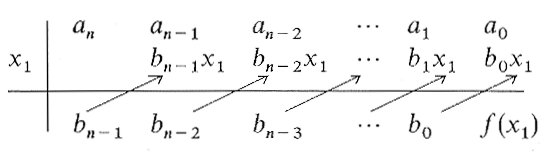
\includegraphics[width=6cm]{./bilder/hornerschema_1.png}\\
		$x_1 \Rightarrow$ Nullstelle (muss erraten werden!!)\\
		oberste Zeile = zu zerlegendes Polynom			
	\end{minipage}
	\begin{minipage}[t]{9cm}
		\textbf{Beispiel:}\\
		$f(x) = x^3-67x-126$\\
		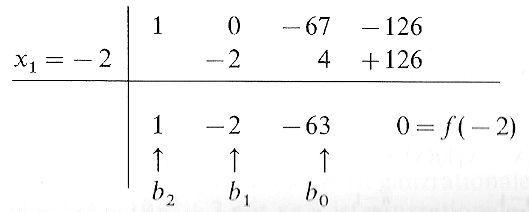
\includegraphics[width=6cm]{./bilder/hornerschema_2.png}\\
		$\Rightarrow f(x) = (x-x_1)(b_2x^2 + b_1x + b_0) = (x+2)(x^2-2x-63)$	
	\end{minipage}